\section{Two-dimensional diffusion equation}
Now we consider two-dimentional diffusion equation; if the diffusion coefficient ($D$) is costant, then  the two-dimensional diffusion equation reduces to the following linear equation:
\begin{equation}
\label{eq:2Dheat}
\frac{\partial \phi(\vec{r},t)}{\partial t}= D \nabla^2 \phi(\vec{r},t)
\end{equation}
and if we assume that $\vec{r}=(x,z)$ it becomes to
\begin{equation}
\label{eq:2DheatOtherForm}
\frac{\partial \phi(x,z,t)}{\partial t}= D \left( \frac{\partial ^2 \phi(x,z,t)}{\partial x^2} +\frac{\partial ^2 \phi(x,z,t)}{\partial z^2} \right).
\end{equation}

\begin{figure}[ht]\centering
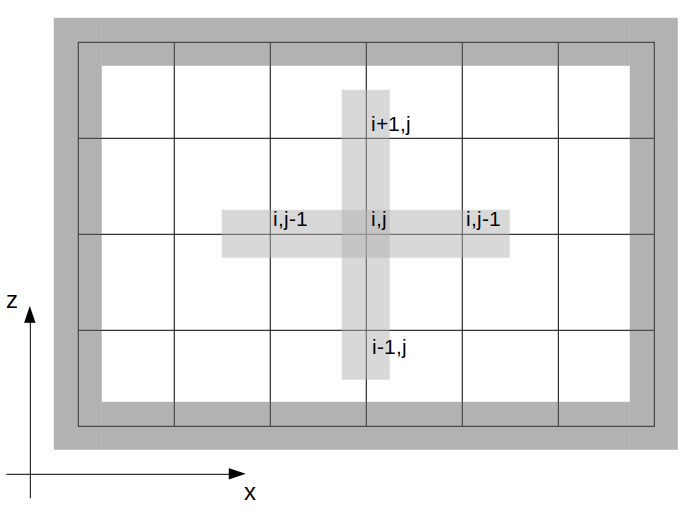
\includegraphics[width=\linewidth]{2d-grid}
\caption{Finite difference discretization of the 2D heat problem}
\label{fig:2d-grid}
\end{figure}

According to the previous explanation on Taylor-series expansion and Linearization of PDEs, if we employ a fully implicit, unconditionally stable discretization scheme as we have done for the 1D equation , equation \ref{eq:2DheatOtherForm} can be written as

\begin{equation}
\frac{\phi^{n+1}_{i,j}-\phi^{n}_{i,j}}{\Delta t} = D ( \frac{\phi^{n+1}_{i,j+1}-2\phi^{n+1}_{i,j}+\phi^{n+1}_{i,j-1}}{(\Delta x)^2} + \frac{\phi^{n+1}_{i+1,j}-2\phi^{n+1}_{i,j}+\phi^{n+1}_{i-1,j}}{(\Delta z)^2} )
\end{equation}
Rearranging terms with $n + 1$ on one side and terms with $n$ on the other side gives
\begin{equation}
\phi^{n}_{i,j} =-s_z \phi^{n+1}_{i+1,j}-s_x \phi^{n+1}_{i,j+1} +(1+2s_z+2s_x) \phi^{n+1}_{i,j} -s_z \phi^{n+1}_{i-1,j}-s_x \phi^{n+1}_{i,j-1}
\label{eq:2Ddescrete}
\end{equation}
As in the 1D case, we have to write these equations in a matrix $A$ and a vector $\vec{b}$. From a practical point of view, this is a bit more complicated than in the 1D case, since we have to deal with “book-keeping” issues, i.e. the mapping of $\phi_{i,j}$ to the entries of a vector $\Phi_k$. 
\\
If a 2D scalar field is to be solved for with an equivalent vector $\Phi$, the nodes have to be numbered continuously, for example as in Figure \ref{fig:2d-grid-mapping}. The derivative versus x-direction is then e.g.

\begin{figure}[ht]\centering
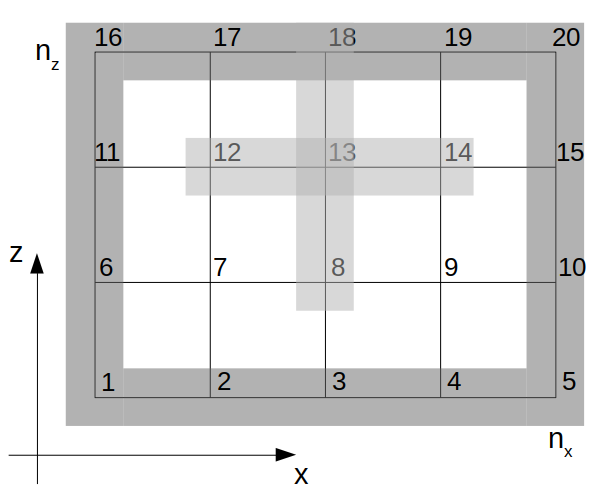
\includegraphics[width=\linewidth]{2d-grid-mapping}
\caption{Numbering scheme for a 2D grid with $n_x = 5$ and $n_z = 4$.}
\label{fig:2d-grid-mapping}
\end{figure}

\begin{equation}
\frac{\partial^2 \phi}{\partial x^2}|_{i=3,j=3}= \frac{1}{(\Delta x)^2}(\Phi_{14}-2\Phi_{13}+\Phi_{12})
\label{eq:grid19x}
\end{equation}
and the derivative versus z-direction is given by
\begin{equation}
\frac{\partial^2 \phi}{\partial z^2}|_{i=3,j=3}= \frac{1}{(\Delta z)^2}(\Phi_{18}-2\Phi_{13}+\Phi_{8})
\label{eq:grid19z}
\end{equation}

If $n_x$ are the number of grid points in x-direction and $n_z$ the number of points in z-direction, we can write equations \ref{eq:grid19x} and \ref{eq:grid19z} in a more general way as:
\begin{equation}
\frac{\partial^2 \phi}{\partial x^2}|_{i,j}= \frac{1}{(\Delta x)^2}(\phi_{(i-1)n_x+j+1}-2\phi_{(i-1)n_x+j}+\phi_{(i-1)n_x+j-1})
\label{eq:gridKx}
\end{equation}
\begin{equation}
\frac{\partial^2 \phi}{\partial z^2}|_{i,j}= \frac{1}{(\Delta z)^2}(\phi_{in_x+j}-2\phi_{(i-1)n_x+j}+\phi_{(i-2)n_x+j})
\label{eq:gridKz}
\end{equation}

As an example, for a $4 \times 5$ grid there are $20$ grid points but $14$ of them are boundary points (located at left, right, top, and bottom) which do not have evolution. There are only $6$ middle points that have evolution in time. Thus, the coefficint matrix $A$ is $20 \times 20$, and on $14$ rows we have just one non-zero element (corresponding to the boundary condition).
\\
According to equation \ref{eq:2Ddescrete}, for a $4 \times 5$ grid, for example, at the boundary points the linear system becomes
%\begin{equation}
\begin{align}
bottom &: \qquad \phi^{n+1}_{1,1}= \phi^{n+1}_{1,2}=\phi^{n+1}_{1,3}=\phi^{n+1}_{1,4}=\phi^{n+1}_{1,5}=\phi_{bottom} \\
top &: \qquad \phi^{n+1}_{4,1}=\phi^{n+1}_{4,2}=\phi^{n+1}_{4,3}=\phi^{n+1}_{4,4}=\phi^{n+1}_{4,5} = \phi_{top} \\
left &: \qquad \phi^{n+1}_{2,1}=\phi^{n+1}_{3,1}=\phi_{left} \\
right &: \qquad \phi^{n+1}_{2,5}=\phi^{n+1}_{3,5}= \phi_{right} \\
\label{eq:2D45boundary}
\end{align}
%\end{equation}
\begin{align}
grid \ point \ 2,2 &:-s_z \phi^{n+1}_{3,2} -s_x \phi^{n+1}_{2,3} +(1+s_z+s_x) \phi^{n+1}_{2,2} -s_z \phi^{n+1}_{1,2} -s_x \phi^{n+1}_{2,1}  = \phi^{n+1}_{2,2} \\
grid \ point \ 2,3 &:-s_z \phi^{n+1}_{3,3} -s_x \phi^{n+1}_{2,4} +(1+s_z+s_x) \phi^{n+1}_{2,3} -s_z \phi^{n+1}_{1,3} -s_x \phi^{n+1}_{2,2}  = \phi^{n+1}_{2,3} \\
grid \ point \  2,4 &:-s_z \phi^{n+1}_{3,5} -s_x \phi^{n+1}_{2,5} +(1+s_z+s_x) \phi^{n+1}_{2,4} -s_z \phi^{n+1}_{1,4} -s_x \phi^{n+1}_{2,3}  = \phi^{n+1}_{2,4} \\
grid \ point \ 3,2 &:-s_z \phi^{n+1}_{4,2} -s_x \phi^{n+1}_{3,3} +(1+s_z+s_x) \phi^{n+1}_{3,2} -s_z \phi^{n+1}_{2,2} -s_x \phi^{n+1}_{3,1}  = \phi^{n+1}_{3,2} \\
grid \ point \ 3,3 &:-s_z \phi^{n+1}_{4,3} -s_x \phi^{n+1}_{3,4} +(1+s_z+s_x) \phi^{n+1}_{3,3} -s_z \phi^{n+1}_{2,3} -s_x \phi^{n+1}_{3,2}  = \phi^{n+1}_{3,3} \\
grid \ point \ 3,4 &:-s_z \phi^{n+1}_{4,4} -s_x \phi^{n+1}_{3,5} +(1+s_z+s_x) \phi^{n+1}_{3,4} -s_z \phi^{n+1}_{2,4} -s_x \phi^{n+1}_{3,3}  = \phi^{n+1}_{3,4} \\
\label{eq:2D45middle}
\end{align}
%\end{equation}
%\end{table*}


and the linear system for the $6$ other points located between the boundaries becomes \ref{eq:2D45middle}.  
\\

%\begin{table*}[ht]
%\begin{equation}

As we explained previously the “book-keeping” issues, i.e. the mapping of $\phi_{i,j}$ to the vector $\Phi_k$ , vectors $\vec{x}$ and $\vec{b}$ become equation \ref{eq:2D45xb}.

\begin{equation}
x= \begin{bmatrix}
	\phi^{n+1}_{1,1} \\ \phi^{n+1}_{1,2} \\ \phi^{n+1}_{1,3} \\ \phi^{n+1}_{1,4} \\ \phi^{n+1}_{1,5} \\ \phi^{n+1}_{2,1} \\ \phi^{n+1}_{2,2} \\ \phi^{n+1}_{2,3} \\ \phi^{n+1}_{2,4} \\ \phi^{n+1}_{2,5} \\ \phi^{n+1}_{3,1} \\ \phi^{n+1}_{3,2} \\ \phi^{n+1}_{3,3} \\ \phi^{n+1}_{3,4} \\ \phi^{n+1}_{3,5} \\ \phi^{n+1}_{4,1} \\ \phi^{n+1}_{4,2} \\ \phi^{n+1}_{4,3} \\ \phi^{n+1}_{4,4} \\ \phi^{n+1}_{4,5} 
\end{bmatrix}
=
   \begin{bmatrix}
	\Phi^{n+1}_{1} \\ \Phi^{n+1}_{2} \\ \Phi^{n+1}_{3} \\ \Phi^{n+1}_{4} \\ \Phi^{n+1}_{5} \\ \Phi^{n+1}_{6} \\ \Phi^{n+1}_{7} \\ \Phi^{n+1}_{8} \\ \Phi^{n+1}_{9} \\ \Phi^{n+1}_{10} \\ \Phi^{n+1}_{11} \\ \Phi^{n+1}_{12} \\ \Phi^{n+1}_{13} \\ \Phi^{n+1}_{14} \\ \Phi^{n+1}_{15} \\ \Phi^{n+1}_{16} \\ \Phi^{n+1}_{17} \\ \Phi^{n+1}_{18} \\ \Phi^{n+1}_{19} \\ \Phi^{n+1}_{20} 
   \end{bmatrix}
    , \qquad \quad
b= \begin{bmatrix}
	\phi^{n}_{1,1} \\ \phi^{n}_{1,2} \\ \phi^{n}_{1,3} \\ \phi^{n}_{1,4} \\ \phi^{n}_{1,5} \\ \phi^{n}_{2,1} \\ \phi^{n}_{2,2} \\ \phi^{n}_{2,3} \\ \phi^{n}_{2,4} \\ \phi^{n}_{2,5} \\ \phi^{n}_{3,1} \\ \phi^{n}_{3,2} \\ \phi^{n}_{3,3} \\ \phi^{n}_{3,4} \\ \phi^{n}_{3,5} \\ \phi^{n}_{4,1} \\ \phi^{n}_{4,2} \\ \phi^{n}_{4,3} \\ \phi^{n}_{4,4} \\ \phi^{n}_{4,5} 
\end{bmatrix}
=
\begin{bmatrix}
	\phi_{bottom} \\ \phi_{bottom} \\ \phi_{bottom} \\ \phi_{bottom} \\ \phi_{bottom} \\ \phi_{left} \\ \Phi^{n}_{7} \\ \Phi^{n}_{8} \\ \Phi^{n}_{9} \\ \phi_{right} \\ \phi_{left} \\ \Phi^{n}_{12} \\ \Phi^{n}_{13} \\ \Phi^{n}_{14} \\ \phi_{right} \\ \phi_{top} \\ \phi_{top} \\ \phi_{top} \\ \phi_{top} \\ \phi_{top} 
\end{bmatrix}
\label{eq:2D45xb}
\end{equation}
And the coefficient matrix, $A$, is \ref{eq:2D45A}. 
\\ 
Now two-dimentional heat equation (\ref{eq:2Dheat}) on a $5 \times 4$ grid reduced to a linear system $A\vec{x}=\vec{b}$, with  $\vec{x}$, $\vec{b}$, and $A$ are given by equations \ref{eq:2D45xb}, \ref{eq:2D45A}. 
\\
This is the way to find the coefficient matrix, and notice that for different boundary conditions we should modify some elements in the coefficient matrix. You can easily understand the pattern in the coefficient matrix, it will help you to build it in your code.
\\
Now that we know how to build the coefficient matrix for two-dimentional problem, it is the time to check what we have orgnized so far. 

\pagebreak

%\afterpage{%
%    \clearpage% Flush earlier floats (otherwise order might not be correct)
%    \thispagestyle{empty}% empty page style (?)
    \begin{landscape}% Landscape page
 	The coefficient matrix, $A$, for a $5 \times 4$ grid is
%\begin{flushleft}
 %   Thus the coefficient matrix, $A$, is
%\end{flushleft}
        \centering % Center table
\begin{equation}
\setcounter{MaxMatrixCols}{20}
\footnotesize{
A = \begin{bmatrix}
    \begin{array}{ccccc|ccccc|ccccc|ccccc}
       1 & 0 & 0 & 0 & 0 & 0 & 0 & 0 & 0 & 0 & 0 & 0 & 0 & 0 & 0 & 0 & 0 & 0 & 0 & 0 \\ %1
       0 & 1 & 0 & 0 & 0 & 0 & 0 & 0 & 0 & 0 & 0 & 0 & 0 & 0 & 0 & 0 & 0 & 0 & 0 & 0 \\ %2
       0 & 0 & 1 & 0 & 0 & 0 & 0 & 0 & 0 & 0 & 0 & 0 & 0 & 0 & 0 & 0 & 0 & 0 & 0 & 0 \\ %3
       0 & 0 & 0 & 1 & 0 & 0 & 0 & 0 & 0 & 0 & 0 & 0 & 0 & 0 & 0 & 0 & 0 & 0 & 0 & 0 \\ %4
       0 & 0 & 0 & 0 & 1 & 0 & 0 & 0 & 0 & 0 & 0 & 0 & 0 & 0 & 0 & 0 & 0 & 0 & 0 & 0 \\ %5
         \hline
       0 & 0 & 0 & 0 & 0 & 1 & 0 & 0 & 0 & 0 & 0 & 0 & 0 & 0 & 0 & 0 & 0 & 0 & 0 & 0 \\ %6
       0 & -s_z & 0 & 0 & 0 & -s_x & (1+2s_z+2s_x) & -s_x & 0 & 0 & 0 & -s_z & 0 & 0 & 0 & 0 & 0 & 0 & 0 & 0 \\ %7
       0 & 0 & -s_z & 0 & 0 & 0 & -s_x & 1+2s_z+2s_x & -s_x & 0 & 0 & 0 & -s_z & 0 & 0 & 0 & 0 & 0 & 0 & 0 \\ %8
       0 & 0 & 0 & -s_z & 0 & 0 & 0 & -s_x & 1+2s_z+2s_x & -s_x & 0 & 0 & 0 & -s_z & 0 & 0 & 0 & 0 & 0 & 0 \\ %9
       0 & 0 & 0 & 0 & 0 & 0 & 0 & 0 & 0 & 1 & 0 & 0 & 0 & 0 & 0 & 0 & 0 & 0 & 0 & 0 \\ %10
          \hline
       0 & 0 & 0 & 0 & 0 & 0 & 0 & 0 & 0 & 0 & 1 & 0 & 0 & 0 & 0 & 0 & 0 & 0 & 0 & 0 \\ %11
       0 & 0 & 0 & 0 & 0 & 0 & -s_z & 0 & 0 & 0 & -s_x & 1+2s_z+2s_x & -s_x & 0 & 0 & 0 & -s_z & 0 & 0 & 0 \\ %12
       0 & 0 & 0 & 0 & 0 & 0 & 0 & -s_z & 0 & 0 & 0 & -s_x & 1+2s_z+2s_x & -s_x & 0 & 0 & 0 & -s_z & 0 & 0 \\ %13
       0 & 0 & 0 & 0 & 0 & 0 & 0 & 0 & -s_z & 0 & 0 & 0 & -s_x & 1+2s_z+2s_x & -s_x & 0 & 0 & 0 & -s_z & 0 \\ %14
       0 & 0 & 0 & 0 & 0 & 0 & 0 & 0 & 0 & 0 & 0 & 0 & 0 & 0 & 1 & 0 & 0 & 0 & 0 & 0 \\ %15
         \hline
       0 & 0 & 0 & 0 & 0 & 0 & 0 & 0 & 0 & 0 & 0 & 0 & 0 & 0 & 0 & 1 & 0 & 0 & 0 & 0 \\ %16
       0 & 0 & 0 & 0 & 0 & 0 & 0 & 0 & 0 & 0 & 0 & 0 & 0 & 0 & 0 & 0 & 1 & 0 & 0 & 0 \\ %17
       0 & 0 & 0 & 0 & 0 & 0 & 0 & 0 & 0 & 0 & 0 & 0 & 0 & 0 & 0 & 0 & 0 & 1 & 0 & 0 \\ %18
       0 & 0 & 0 & 0 & 0 & 0 & 0 & 0 & 0 & 0 & 0 & 0 & 0 & 0 & 0 & 0 & 0 & 0 & 1 & 0 \\ %19
       0 & 0 & 0 & 0 & 0 & 0 & 0 & 0 & 0 & 0 & 0 & 0 & 0 & 0 & 0 & 0 & 0 & 0 & 0 & 1 \\ %20
   \end{array}
    \end{bmatrix}
\label{eq:2D45A}
}
\end{equation}

 	The coefficient matrix, $A$, for a $4 \times 5$ grid is
%inja
\begin{equation}
\setcounter{MaxMatrixCols}{20}
\footnotesize{
A = \begin{bmatrix}
    \begin{array}{cccc|cccc|cccc|cccc|cccc}
       1 & 0 & 0 & 0 & 0 & 0 & 0 & 0 & 0 & 0 & 0 & 0 & 0 & 0 & 0 & 0 & 0 & 0 & 0 & 0 \\ %1
       0 & 1 & 0 & 0 & 0 & 0 & 0 & 0 & 0 & 0 & 0 & 0 & 0 & 0 & 0 & 0 & 0 & 0 & 0 & 0 \\ %2
       0 & 0 & 1 & 0 & 0 & 0 & 0 & 0 & 0 & 0 & 0 & 0 & 0 & 0 & 0 & 0 & 0 & 0 & 0 & 0 \\ %3
       0 & 0 & 0 & 1 & 0 & 0 & 0 & 0 & 0 & 0 & 0 & 0 & 0 & 0 & 0 & 0 & 0 & 0 & 0 & 0 \\ %4
         \hline
       0 & 0 & 0 & 0 & 1 & 0 & 0 & 0 & 0 & 0 & 0 & 0 & 0 & 0 & 0 & 0 & 0 & 0 & 0 & 0 \\ %5
       0 & -s_z & 0 & 0 & -s_x & 1+2s_z+2s_x & -s_x & 0 & 0 & -s_z & 0 & 0 & 0 & 0 & 0 & 0 & 0 & 0 & 0 & 0 \\ %6
       0 & 0 & -s_z & 0 & 0 & -s_x & 1+2s_z+2s_x & -s_x & 0 & 0 & -s_z & 0 & 0 & 0 & 0 & 0 & 0 & 0 & 0 & 0 \\ %7
       0 & 0 & 0 & 0 & 0 & 0 & 0 & 1 & 0 & 0 & 0 & 0 & 0 & 0 & 0 & 0 & 0 & 0 & 0 & 0 \\ %8
       \hline
       0 & 0 & 0 & 0 & 0 & 0 & 0 & 0 & 1 & 0 & 0 & 0 & 0 & 0 & 0 & 0 & 0 & 0 & 0 & 0 \\ %9
       0 & 0 & 0 & 0 & 0 & -s_z & 0 & 0 & -s_x & 1+2s_z+2s_x & -s_x & 0 & 0 & -s_z & 0 & 0 & 0 & 0 & 0 & 0 \\ %10
       0 & 0 & 0 & 0 & 0 & 0 & -s_z & 0 & 0 & -s_x & 1+2s_z+2s_x & -s_x & 0 & 0 & -s_z & 0 & 0 & 0 & 0 & 0 \\ %11
       0 & 0 & 0 & 0 & 0 & 0 & 0 & 0 & 0 & 0 & 0 & 1 & 0 & 0 & 0 & 0 & 0 & 0 & 0 & 0 \\ %12
       \hline
       0 & 0 & 0 & 0 & 0 & 0 & 0 & 0 & 0 & 0 & 0 & 0 & 1 & 0 & 0 & 0 & 0 & 0 & 0 & 0 \\ %13
       0 & 0 & 0 & 0 & 0 & 0 & 0 & 0 & 0 & -s_z & 0 & 0 & -s_x & 1+2s_z+2s_x & -s_x & 0 & 0 & -s_z & 0 & 0 \\ %14
       0 & 0 & 0 & 0 & 0 & 0 & 0 & 0 & 0 & 0 & -s_z & 0 & 0 & -s_x & 1+2s_z+2s_x & -s_x & 0 & 0 & -s_z & 0 \\ %15
       0 & 0 & 0 & 0 & 0 & 0 & 0 & 0 & 0 & 0 & 0 & 0 & 0 & 0 & 0 & 1 & 0 & 0 & 0 & 0 \\ %16
       \hline
       0 & 0 & 0 & 0 & 0 & 0 & 0 & 0 & 0 & 0 & 0 & 0 & 0 & 0 & 0 & 0 & 1 & 0 & 0 & 0 \\ %17
       0 & 0 & 0 & 0 & 0 & 0 & 0 & 0 & 0 & 0 & 0 & 0 & 0 & 0 & 0 & 0 & 0 & 1 & 0 & 0 \\ %18
       0 & 0 & 0 & 0 & 0 & 0 & 0 & 0 & 0 & 0 & 0 & 0 & 0 & 0 & 0 & 0 & 0 & 0 & 1 & 0 \\ %19
       0 & 0 & 0 & 0 & 0 & 0 & 0 & 0 & 0 & 0 & 0 & 0 & 0 & 0 & 0 & 0 & 0 & 0 & 0 & 1 \\ %20
   \end{array}
    \end{bmatrix}
\label{eq:2D54A}
}
\end{equation}

\end{landscape}



Like what we have done for the one-dimentional part, here we can ignore the boundary points in the solution vector (all $\phi_{top}$, $\phi_{bottom}$, $\phi_{left}$, and $\phi{right}$) and just solve the equation for the evolving middle ponits. Like befor we consider the boundary conditions in a boundary condition vector ($\vec{b.c.}$). For two dimensional case, we can rewrite the linear system as:
\begin{equation}
A'\vec{x'}=\vec{b}+\vec{b.c.}
\end{equation} 
where vectors $\vec{x'}$, $\vec{b'}$, and $\vec{b.c.}$ are:
\begin{equation}
\vec{x'}=\begin{bmatrix}
 \Phi^{n+1}_{7} \\ \Phi^{n+1}_{8} \\ \Phi^{n+1}_{9} \\  \Phi^{n+1}_{12} \\ \Phi^{n+1}_{13} \\ \Phi^{n+1}_{14}
\end{bmatrix}
\quad
\vec{b'}=\begin{bmatrix}
 \Phi^{n}_{7} \\ \Phi^{n}_{8} \\ \Phi^{n}_{9} \\  \Phi^{n}_{12} \\ \Phi^{n}_{13} \\ \Phi^{n}_{14}
\end{bmatrix}
\quad
\vec{b.c.}= \begin{bmatrix}
+s_{z} \phi_{bottom} +s_{x} \phi_{left} \\ +s_{z} \phi_{bottom} \\ +s_{z} \phi_{bottom} + s_{x} \phi_{right}  \\ +s_{z} \phi_{top} + s_{x} \phi_{left} \\ +s_{z} \phi_{top} \\ +s_{z} \phi_{top} + s_{x} \phi_{right}
\end{bmatrix}
\end{equation}
and coefficient matrix $A'$ is \ref{eq:coefmatrix2dA'}

\begin{table*}[ht]
\begin{equation}
A' = \begin{bmatrix}
	   (1+2s_z +2 s_x) & -s_x & 0 & -s_z & 0 & 0  \\
   	   -s_x & (1+2s_z +2 s_x) &-s_x & 0 & -s_z & 0   \\
   	   0 & -s_x & (1+2s_z +2 s_x) &-s_x & 0 & -s_z   \\
  	   -s_z & 0 & -s_x & (1+2s_z +2 s_x) &-s_x & 0   \\
   	   0 & -s_z & 0 & -s_x & (1+2s_z +2 s_x) &-s_x  \\
   	   0 & 0 & -s_z & 0 & -s_x & (1+2s_z +2 s_x)  \\
     \end{bmatrix}
     \label{eq:coefmatrix2dA'}
\end{equation}
\end{table*}


